\documentclass[conference]{IEEEtran}

\hyphenation{op-tical net-works semi-conduc-tor}

\usepackage{syntonly}
%\syntaxonly
\usepackage{amsmath}
\usepackage{url}
\usepackage{cite}

%------------------------------------------------------------------------------
%   list
%------------------------------------------------------------------------------
\usepackage{enumitem}
\usepackage{fancyvrb}
\usepackage{framed}
%------------------------------------------------------------------------------
%   algorithm
%------------------------------------------------------------------------------
\usepackage{algorithm, algorithmicx}
\usepackage[noend]{algpseudocode}

%------------------------------------------------------------------------------
%   paste code
%------------------------------------------------------------------------------
\usepackage{listings}
\lstset{showstringspaces=false}
%\lstdefinestyle{showspaces=false}
\usepackage{courier}
%\lstset{basicstyle=\footnotesize\ttfamily,breaklines=true}
\lstset{basicstyle=\normalfont\ttfamily,breaklines=true,showspaces=false}
%\lstset{framextopmargin=50pt,frame=bottomline}

%------------------------------------------------------------------------------
%   graph
%------------------------------------------------------------------------------
\usepackage{tikz}

%------------------------------------------------------------------------------
%   url
%------------------------------------------------------------------------------
\usepackage{hyperref}

%------------------------------------------------------------------------------
%   pic
%------------------------------------------------------------------------------
\usepackage{graphicx}
\DeclareGraphicsExtensions{.pdf,.png,.jpg}
\graphicspath{{picture/}}

%------------------------------------------------------------------------------
%   title
%------------------------------------------------------------------------------
\title{Are You Coding Safely? A Guideline for Web Developers}

\author{\IEEEauthorblockN{Chun-Chan (Bill) Cheng}
\IEEEauthorblockA{Department of Computer Science and Engineering\\
Texas A\&M University\\
Email: aznchat@tamu.edu }
\and
\IEEEauthorblockN{Chia-Cheng (Jeremy) Tso}
\IEEEauthorblockA{Department of Computer Science and Engineering\\
Texas A\&M University\\
Email: jjjjj222@tamu.edu}}

\begin{document}
%------------------------------------------------------------------------------
%   begin
%------------------------------------------------------------------------------
\maketitle

%\section{Introduction}
%Since the invention of the World Wide Web (WWW) by Tim Berners-Lee, it has been drastically gaining popularity in the world in the last two decades. The WWW provides a vast source of information of almost every types, ranging from stock databases to your every day weather report. Yet, in order to access the WWW, a browser is required. So came the different browsers from different cooperates and different web applications associated with different browsers we are using today. In fact, due to the proliferation of hand-holding devices in the past five years, the ubiquitous accessibility of the web browser has been a norm for today's applications. Now basically every service supports an on demand access through all kinds of devices.
%
%Web applications have many advantages over traditional ones which require installation. First of all, it works on every platform as long as there's a web browser. This takes makes developing web application a lot easier for engineers, since once a job done, it works everywhere. No more customization for different platforms. No more separated team members. Secondly, application can be patched instantly, which people usually ignore. No more asking for user to upgrade Last of all, web applications are fast deployable, fast prototype, light-weighted and is easy to get feed backs from the market.
%
%Due to these advantages, tons of frameworks and languages, from server side php to client side html, emerged for web developing. With the help of new language, new framework building an website or web application becomes very easy. Anybody can build a web application by just learning the basic of these languages. On the other hand, frameworks help you fasten the production of your web application by including third party libraries and various helpers that assist you through the development process. With the help of frameworks and new languages, no more tedious work to read through all the manual script to just understand one of the languages to write a web application.
%
%Despite the glorious future for web development, there are still many pitfall. While engineers are busy on bringing out all the functionalities, they may not have time to work on security. Which may lead to devastating consequences. Our proposal here is to provide some simple, clear but also useful guidelines to help engineer code with "good habits"
%
%Note that our goal here is not to cover every vulnerabilities, which is intuitively impossible. Our goal here is to cover as many problems as possible with minimal efforts. One might think this is not good enough. However, the concept of security is that if the value of the data in your website is less than the effort that one needs to break in, or in other words, the attacker would need to put a time that is not worth to steal your data, then, in this case, the protection should be sufficient.
%
%According to the ``Pareto principle'' , or known as the 80-20 law, most of the easy vulnerabilities should be able to eliminated, if one avoids most of vulnerability by eliminating bad coding style. It is not likely to notice every single problem without the help of scanner or static analyzer, however, by just following the guidelines of the different frameworks and languages that we propose, we believe that security breaches in the web applications may be minimized.
%
\section{Introduction}
With the proliferation of hand-holding devices,
the ubiquitous accessibility has been a norm for today's applications.
Basically every service today supports on-demand access through all kinds of devices,
and users should be able to use whatever service they like to receive.
%ranging from Macbook, iPad, to Windowns phone.
%users should be able to use Android, iOS, Windows, or Linux as they wish.
To meet this requirement, more and more service providers tend to roll
out their product as a
web application.

Web applications have many advantages over the traditional download-and-install ones:
First of all, they work on every platform as long as there's a web browser.
This takes a lot of pains off software engineers, because once a job is done, it works everywhere
-- no more customization or porting for different platforms.
%No more seperated team members.
Secondly, web applications can be patched instantly.
Every user will have the same version of application at any given time,
and it relieves engineers from
tiresome backward-compatible requirements.
%which people usually ignore.
%No more asking for user to upgrade
%Thirdly,
Moreover,
applications can be used immediately without tedious download-install process.
This fast deployment, fast prototype, and light-weighted characteristics
greatly facilitates the project development in terms of
increasing time-to-market speed.
It also helps service providers get the instant
feedback from market, and thus alter their direction of strategy accordingly in early stage.

Due to these advantages, lots of programming languages with their frameworks have
%, from server side php to client side html,
emerged for web development. With the help of these new tools,
building a web application is not an ``geek job'' anymore:
%becomes very easy.
anybody can build a web application by simply following some basic tutorials.
%On the other hand, frameworks help you fasten the production of your web
%application by including third party libraries and various helpers that assist
%you through the development process. With the help of frameworks and new languages,
%no more tedious work to read through all the manual script to just understand one
%of the languages to write a web application.
However, although these tools are easy to use,
%Despite the glorious future for web development,
%there are many pitfalls.
they have many pitfalls as well. For instance, in PHP 4.2.0 or lower, PHP had global variable that could be access 
any where in the application. Since PHP does not require variables to be initialized when declared, if programmers
do not take steps to protect this variable. It is likely that this variable may be compromised by malicious user by
using various of techniques, such as script injections.
%They treat

Once a developer steps on some of them, the newly-built web application could
be another puppets controlled by malicious hackers. Continuing the example stated above, if the malicious user
decides to gain root access to the server folder of your website by using the compromised variable. See the example code below:
\begin{framed}
\begin{verbatim}
if (authenticated_user()) {
    $authorized = true;
}

Program continues on....

if ($authorized) {
    Sensitive_Data();
}
\end{verbatim}
\end{framed}
%TODO: example

Since \texttt{\$authorize} can be initialized even without \texttt{authenticated\_user()} and it has not been initialized to false in the beginning. Attacker
can take advantage of this, defining \texttt{\$authorized} through various techniques, for example, defining the variable \texttt{\$authorized} through \texttt{register\_globals}. 
Boom! Your website is compromised, all the sensitive data are exposed to the attacker!

To prevent this from happening, we want to provide some simple, clear but
useful guidelines to help programmer code with ``good habits".
Normally, while engineers are busy on bringing out all the functionalities,
they do not have enough time to work on security. By following our guidelines,
they only have to pay a little extra attention, while getting a more secure application.
%the application can be more security with some
%which may lead to devastating consequences.

Note that our goal here is not to cover every vulnerabilities, which is intuitively impossible.
Our goal here is to cover as many problems as possible with minimal efforts.
You might think it's not good enough.
However, the concept of security is that if the value of the data in your website
least than the effort that one need to break in, then, in this case,
the protection should be sufficient.
%Due to its advantages, tons of framework/language emerge.
%
%with the help of new language, new framework
%building an website/web application becomes very easy.
%everybody can code
%
%And there are many more pitfall
%While engineer are busying on bring out all the functionalities,
%they may not have time to work on security.
%
%Despite the glorious future for web development, there are still many pitfall. While engineers are busy on bringing out all the functionalities, they may not have time to work on security. Which may lead to devastating consequences. Our proposal here is to provide some simple, clear but also useful guidelines to help engineer code with "good habits"
%
%Note that our goal here is not to cover every vulnerabilities, which is intuitively impossible. Our goal here is to cover as many problems as possible with minimal efforts. One might think this is not good enough. However, the concept of security is that if the value of the data in your website is less than the effort that one needs to break in, or in other words, the attacker would need to put a time that is not worth to steal your data, then, in this case, the protection should be sufficient.
%
%According to the ``Pareto principle'' , or known as the 80-20 law, most of
%the easy vulnerabilities should be able to eliminated, if one
%avoids most of vulnerability by eliminating bad coding style. It is not likely
%to notice every single problem without the help of scanner or static analyzer, however,
%by just following the guidelines of the different frameworks and languages that we
%propose, we believe that security breaches in the web applications may be minimized.

%problem statement,
%proposed technique/solution,
%a survey of related work(and comparison),
\section{Problem Statement}
Engineers have to face many pitfalls while working on an web application, such as
various framework structures and different language behaviors.
%Different servers, different languages, and different frameworks.
%such as buffer overflow, cross-site scripting, SQL injection,
On developing,
they are often too busy to pay attention on securities.
This phenomenon leads to vulnerable sites,
which could be used as medium to carry out malicious behavoirs by others.
%to resolve this issue.

\section{Proposed Solution}
Our target here is to provide some simple, clear but useful guidelines
to help engineer code with "good habits", and thus
eliminate most of vulnerabilities with minimal efforts.

%Note that our goal here is not to cover every vulneribilities, which is intuitively impossible.
%20/80 law
%most of the easy vulneribilities should be able to eliminated.
%avoid most of vulnerability by void bad coding style.
%
%It's not likely to notice every single problem without the help of scanner or static analyzer,
%however,
%
%
\section{Related Work}
Different web application vulnerability have been proposed before. In this section we will include some of the most common 
vulnerabilities that have been proposed till now. First of all, one of the most famous and most ancient attack is the sql injection 
attack which was first documented by Jeff Forristal, more know by the name of rain forest puppy \cite{Jeff}. 
 SQL injection vulnerabilities have been described as one of the most serious threats for Web applications \cite{Aucsmith} \cite{TO}. 
 In 2006, Professor Halfond classified the SQL injection attacks and proposed some countermeasure \cite{halfond06mar}.

Secondly, another famous web application attacks is the Cross Site Scripting(CSS). 
Cross-site scripting carried out on websites accounted for roughly 84\% of all security vulnerabilities documented by Symantec as of 2007\cite{symantec}. 
Cross-site scripting (XSS) attacks target an application's users by injecting code, usually a client-side script such as JavaScript, into a Web application's output. 
These attacks can cause small petty security ricks to devastating data theft depending on how sensitive are the data in the websites.

Third of all, the session management and user authentication. Web applications have to handle user authentication and establish sessions to keep track 
of each user's requests as HTTP does not provide this capability. If there is a breach in the session management of 
a web application, the attacker can then steal the user cookie and impersonate this person on the web. 
However, cookies are not accessible via non-HTTP methods, such as calls via JavaScript, by using document.cookie, and therefore cannot be stolen easily via cross-site scripting\cite{symantec}.

Last of all, the insecure direct object reference. If the web application design does not have mistake-proofing mechanism and assumes that users will always follow the application rules, 
then it is likely that a user may accidentally jump into a page that it was not granted access. This is the benign security breach, since the user may not want to steal any information, 
but what if a malicious user starts stealing the information or to make things worse, a hacker that can read the URL or can guess the hidden field of the URL\cite{Michael}. 
If this happens, you web application can be in big trouble.  \cite{Test}.

\section{Configuration}
In the report we will mainly focus on the things stated below
because it's the most common setup. In the final report we will do case testing for the things we have proposed.
Configuring the environment is tedious but it is crucial. In web application, there are mainly three parts to configure
which are the system (linux), the server (apache), and the language that you are writing your web application on.
\section{Setup Local Host Website}
We will demonstrate the possible attacks if the system or any file is not configured correctly with a website we have setup. This is intended to be a raw website without any defense against any attacks. The below is the screen shot of the basic website format. All screenshots example in the followings are all attacks of this localhost website
\begin{figure}[h]
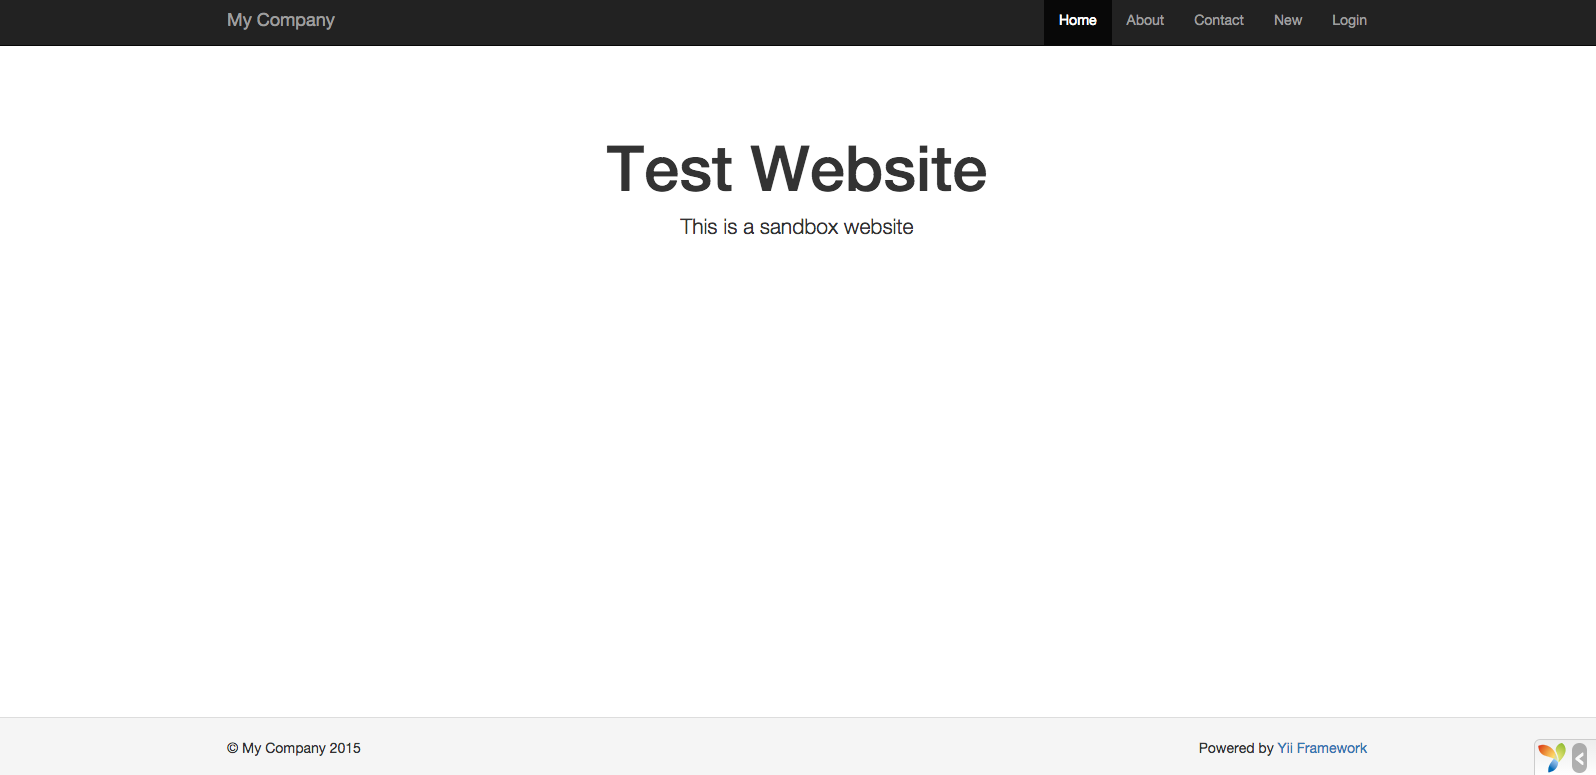
\includegraphics[width=8cm, height=4cm]{yii}
\centering
\caption{Localhost website}
\end{figure}
\section{Apache Server Setup}
Apache server is now the most dominant http server. We can see in \cite{ApachePopularity} that till November 28 2015, Apache still had $55.7\%$ of the market share. So we will focus on the configuration for the Apache server.

\subsection{Options}
If this variable was turned on, we can see the directory of the web server. This is really not a good idea to let users see your directories. You should always check before releasing the product. Attackers could gain a lot information just by looking at this. For example, looking at this directory, attackers can now know that this is a MVC model. Attackers could easily hijack the model or controller and send the user to another malicious cite.
\begin{figure}[h]
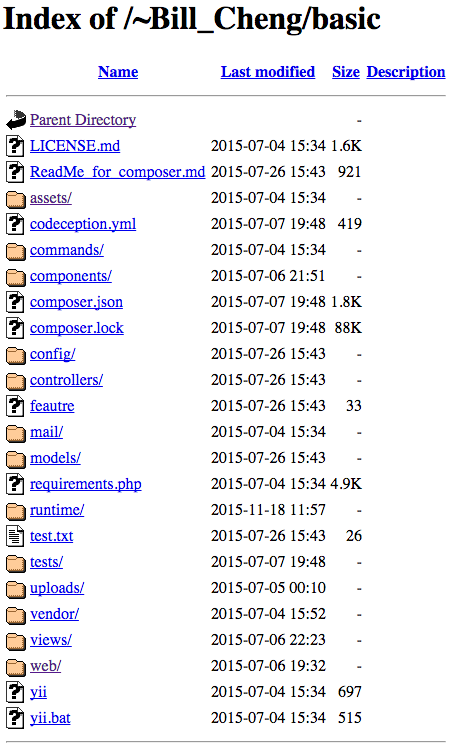
\includegraphics[width=4cm, height=6cm]{options_none}
\centering
\caption{Directory of the localhost server.}
\end{figure}

\subsection{AllowOverride}
Next, we move on to AllowOverride variable. This is an important variable because, if this is set to All, all the configuration you have configured in the APACHE file can be overridden by this file. This main purpose was used because different file needed different configuration for the APACHE server, however it strongly recommended you turn this off. If attackers gain access to this file, you apache server may be in danger too.  For the example: when a user links to this server from google or facebook, it is automatically rendered to a new webpage which can be malicious.

\lstset{escapeinside={<@}{@>}}
\begin{lstlisting}[ basicstyle=\small\ttfamily]
RewriteEngine On
RewriteCond %{HTTP_REFERER} .*google.* [OR]
RewriteCond %{HTTP_REFERER} .*facebook.* [OR]
RewriteRule ^(.*)$<@\textcolor{red}{http://malwarewebsite.com}@>
\end{lstlisting}

\subsection{ServerSignature}
This signature shows the version of APACHE and PHP, which is not an good idea because there are known vulnerabilities for out of date APACHE version which can be exploited.
\begin{figure}[h]
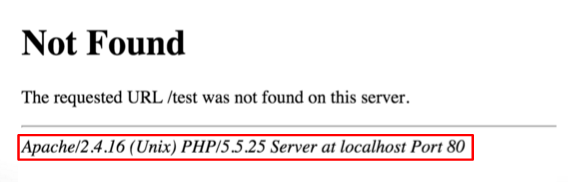
\includegraphics[scale=0.3]{serversignature}
\centering
\caption{The red box is the version number of apache and php.}
\end{figure}


\section{PHP.ini}
We will focus mainly on PHP, which covers more than $80\%$ \cite{PHPusuage} of the server side languages. We have done the initial
survey of the PHP, which includes the php.ini setup.
PHP.ini file is an important configuration file for PHP. You declare all the configuration settings in this file. Since the php.ini file is read each time PHP is initialized, it is important that
PHP developer know the basic security configuration of the PHP.ini file. Below we will give some basic guidelines for developers on what to set to the environment variable in the PHP.ini
to prevent petty attacks. Even though this configuration won't by itself fend off a determined attacker, but it will lower visibility to attacks that rely on simple techniques to scan for vulnerable targets\cite{phpini}.
 
\subsection{expose\_php}
\texttt{Expose\_php}, when turned on will tell the web server to send back the \texttt{X-Powered-By} header, in other words, \texttt{Expose\_php} will return back in every request what version of PHP is installed.

\begin{figure}[h]
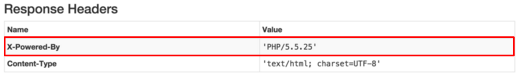
\includegraphics[scale=0.5]{exposephp}
\centering
\caption{The red box is the version number of php.}
\end{figure}


\subsubsection{Vulnerability}
If a web application is using a PHP version that is out of date or using a PHP version with known vulnerabilities, malicious attackers can exploit this vulnerability causing the web application to be 
unsecure\cite{exposephp}.

\subsubsection{Recommendation}
Setting the \texttt{Expose\_php} to \texttt{off} is recommended. Even though determined attackers can still get the version of your php but it would take them more time trying to achieve this. In addition,
 the web application can stand up to simple attack scanning for specific version of php vulnerabilities. In conclusion, it is always better to set \texttt{Expose\_php} to \texttt{off} than never.
 
\subsection{post\_max\_size}
The environment variable \texttt{post\_max\_size} is the variable that sets the size that \texttt{\$\_POST} method can send over to the server.
\subsubsection{Vulnerability}
If this environment variable is not set to a realistic value, for example, if you set the value to 1024 MB, then you are giving attackers permission to put your server at stress by sending oversized POST request.\cite{postmaxsize}
\subsubsection{Recommendation}
By setting a realistic value here you can mitigate some of the damage by those attacks. This protection allows you to limit the maximum size POST request that PHP will process.

\subsection{display\_errors}
Display\_error is often forgotten when developers release their product. It is always not good to let user see the error. First of all, it's annoying. Second of all, it is really dangerous because there might be a logic flaw in your system which is a vulnerabilities. 
\begin{figure}[h]
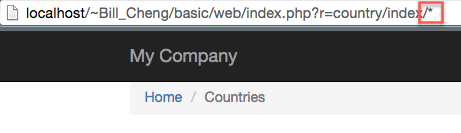
\includegraphics[scale=0.45]{displayerror}
\centering
\caption{Attackers can detect sql injection vulnerabilities by inserting ``/*" to the end of the url}
\end{figure}

If a website is vulnerable to sql injection and displays error back to the users, the users will receive the following errors when \texttt{display\_errors} is turned on: \\\\
\texttt{You have an error in your SQL syntax; check the manual that corresponds to your MySQL server version for the right syntax to use near `/* ORDER BY $\dotso$'}

\section{String I/O}
The string exploit occurs when the submitted data of an input string is evaluated as a command by the application. In this way, the attacker could execute code, read the stack, or cause a segmentation fault in the running application, causing new behaviors that could compromise the security or the stability of the system.

\subsection{Input}
We should never trust a user, and we should never think that our web application is just a small project. If you are dealing with sensitive information, always keep in mind that not all user have the knowledge in security, so they might use the same password as their bank account. So when a user gives a input we should validate it and filter it. For example, if it is a password input, we should give it white list, only the characters in the white list is allowed. If the input is supposed to be input of a dropdown list, checkbox, radio button, we should validate if the value is the value we intend to receive. Otherwise we reject them.

\subsubsection{Server-side vs Client-side Validation}
A common mistake that developer make is only validating the user input on the client side with javascript. This can easily be bypass when user disables javascript. Validation on the user side are beneficial but can not provide full security. In addition, the server-side validation routine will always be effective irrespective of the state of JavaScript execution on the browser. As a best practice input validation should be performed both on the client side as well as on the server side.


\subsubsection{White List}
Application whitelisting is a computer administration practice used to prevent unauthorized programs from running. The purpose is primarily to protect computers and networks from harmful applications, and, to a lesser extent, to prevent unnecessary demand for resources\cite{whitelist}. It's recommended to use whitelist when users submit a password and username.


\subsubsection{Escape}
There are two ways for developers to handle escape in user inputs. The first way is when user sends data to server developers should escape it and then store it into database. Second way is for developers to store data as it is and escape it when data are send to users.

There are pros and cons to these two different escaping approaches. The former one is a lot easier, escaping and then saving data to database. However, let's suppose an attacker figures out the flow in our website and manages to avoid escaping. Then the developer will have a problem of finding all data that was stored to the database unescaped.

The latter just stores data as it is but escape it once developer sends it to user. In this case, even if someone finds the flow of the  website all the developers has to do is fix the bug, since the system already assumes that data saved in database is not escaped.

Although second approach seems easier but it is a lot more prone to error. Suppose we generate HTML on server and send it to user and then decide to switch to just sending content to user via ajax, it is easy to forget that we need to escape all the data before sending it to user or implementing new API.

To wrap things up, there are two common solutions. 1) Escape the data before storing it. 2) Store two copies of the data, one escaped, and one raw.
%pro: more general,
%con: hard to do it right
%escape function:
%1. php
%2. python

\subsection{Output}
In addition to validating all of the data the application receives, developers should also follow similar processes for the data the application will output. Some attacks such as Cross Site Scripting(XSS) can take advantage of poorly validated output to attack unsuspecting end users through the application. There are three main issues associated with output validation that developers should alway aim to keep an eye on in your application; they are data encoding, data format and data length\cite{outputvalidation}.

\subsubsection{XSS}
In a cross-site scripting (XSS) attack, the attacker injects malicious code into a web page that then runs malicious client-side script. When a user visits the infected web page, the script is downloaded to, and run from, the user's browser. This can lead to account hijacking, spread of web worms, access to browser history and clipboard contents, remotely controlling the browser, or scanning and exploiting website vulnerabilities\cite{XSS}.

\subsubsection{HTML Encoding}
A quick and straightforward way to prevent XSS is by encoding HTML responses. In fact, PHP has a library \texttt{htmlspecialchars}\cite{htmlspecialchars} that converts special characters to HTML entities. However, HTML encoding does not prevent developers from all XSS attacks. For example, suppose web server generate client side javascript , the server automatically sends html encoded scripts to the client side, in this case html encode will not stop injected script from executing.

Despite it not being able to prevent all XSS, encoding is still the correct approach, but developers would need context-sensitive encoding\cite{contextencoding}. This is when the server can recognize which context that is about to be sent to a rendering page is a unintended script or not.
%reason: avoid XSS
%method: escape?
%how to escape html?

\subsection{Conclusion}
Developers should bear in mind that not all users know about web security. So users may use the same password over multiple websites and not all website have the same security levels. If your web application becomes breached and username and passwords are stolen. Then the users are in immediate danger that all their other accounts may be hacked. Due to this, it is always a necessity to put most of your effort on the the string inputs and outputs.

%------------------------------------------------------------------------------
%   
%------------------------------------------------------------------------------
\section{Database Access}
Almost all the information are stored in database today,
including users' account/password, their data, and their
personally identifiable information (PII).
Therefore,
datacases are often the main target of attackers.
Among all the atacks, SQL injection is the most common one.
We focus on MySQL here because it's the LAMP \cite{LAMP} boudle is widely used.
\\\\
%\subsection{setup}
%account, password, access
%information.schema?
%access permission?
Setting up database correctly, as other part of the system, is a necessity.
We will discuss that later.
Another key point is to use the specialized functions provided by databases
instead of general ones. For example, using proposed function can effectively
avoid some SQL injection. Below is an exmple in Python:
\\\\
%\subsection{R/W}
%use proposed: avoid sql injection
%python example:
%cite: https://www.python.org/dev/peps/pep-0249/ Python Database API
%.execute ( operation [, parameters ])
%Prepare and execute a database operation (query or command).
%cur example: http://initd.org/psycopg/docs/usage.html#query-parameters
Don't:
\begin{lstlisting}[language=python]
cursor.execute("SELECT * FROM table WHERE id=%s" % (id));
\end{lstlisting}
Do:
\begin{lstlisting}[language=python]
cursor.execute("SELECT * FROM table WHERE id=%s" , id);
\end{lstlisting}
The first one is normal format string construction in python.
placeholder \%s will be replaced by id,
and the whole query will be executed.
Apparently, there is an injection problem.
%injection problem
On the other hand,
the second one use proposed function with paramters.
It pre-computes the query and apply the whole \%s directly for comparison.
%pre-compute
If somebody tries to perform an SQL injection, the system will block it automatically.
\begin{lstlisting}[language=python]
Warning: Truncated incorrect DOUBLE value: '1 OR 1=1'
\end{lstlisting}


%\subsection{data}
%django
%https://docs.djangoproject.com/en/1.8/topics/auth/passwords/
%http://stackoverflow.com/questions/749682/django-passwords Django Code

%https://en.wikipedia.org/wiki/Rainbow_table Rainbow table
%1. hash passward
%2. add salt while hashing, rainbow table


%------------------------------------------------------------------------------
%   crypto
%------------------------------------------------------------------------------
\section{Cryptographic Utilities}
%Needless to say, the
%network
Everybody knows that it's important to encrypt data while sending them over the internet,
yet not everybody does it right.
As the technologies of cryptography evolving,
they become more and more complicated.
%It's not the simple one-key-one-algorithm anymore.
Normally, in an encrpyted communication, there are more the 1 keys involved,
along with parameters, nonces, and different kinds of operation modes;
some of them should be kept secret, while others are not;
some of them can be reuse, while others must change every time.
%some are public, some should be kept secret,
%set up, %nonce, %some
It's overwhelming for most of developors, and even an expertise might sometimes get it wrong.
\\\\
%key, function, implementatino, nonce.
One of the exmples is the famous Sony PlayStation 3 issue \cite{PS3_Jailbreak}:
Sony used ECDSA \cite{ECDSA} but didn't change the ephemeral key, so the
private was calculated easily.
%cite https://en.wikipedia.org/wiki/PlayStation_Jailbreak
%cite https://en.wikipedia.org/wiki/Elliptic_Curve_Digital_Signature_Algorithm
Other well-known example is the
side channel attack such as differential power analysis \cite{differential}:
%cite https://en.wikipedia.org/wiki/Side-channel_attack
The implementation is correctly, but functional correctness is not sufficient to
be crpytographically secure.
%For the
%lack of knowledge
%looks fine but indeed not
\\\\
%cite http://www.nist.gov/ NIST
%cite https://www.owasp.org/index.php/Guide_to_Cryptography OWASP guide
%cite http://csrc.nist.gov/groups/ST/toolkit/documents/dss/NISTReCur.pdf NIST ecc recommendation
To support developors, we concluded the following guildlines:
%Three most important concepts
\begin{enumerate}[label=\textbf{\arabic*.}]
    \item
Always encrypt the communication. You never know what information would help hackers
break into your syatem, even if they appear to be harmless.
    \item
Use well-known standard, don't invent the encrpytion algorithm.
%TODO: NIST \cite{NIST}
%TODO: NXP mifare \cite{mifare_break}
    \item
%use the good one
Use the up-to-date standard.
Some algorithms such as md5 have been proved to be unsafe \cite{md5_break}.
    \item
Use libraries, don't implement algorithm yourself.
(even  RNG)
    \item
Use it right,
follow guides carefully for setup (such as those published by NIST \cite{NIST}).
\end{enumerate}

We will provide a more completet list of recommended functions,
for hash, symmetric and assymetric encropyion,
in many common web-debelop languages
in the final report.

%\subsection{SHA, AES, RSA, ECC?}
%provide some python function
%%cite: https://docs.python.org/2/library/hashlib.html#module-hashlib Python hashlib
%
%%cite: https://en.wikipedia.org/wiki/Cryptographic_hash_function#Cryptographic_hash_algorithms
%Don't use MD5, SHA-1
%Use SHA-2
%%cite: https://en.wikipedia.org/wiki/SHA-2
%
%good function for
%1. hash
%2. encrpytion
%3. randeon number geneerator
%%https://pypi.python.org/pypi/pycrypto
%python crypto function
%
%key strength match
%because the weakest part
%
%\subsection{SSL}
%library and their setup?


%------------------------------------------------------------------------------
%   
%------------------------------------------------------------------------------
\section{Useful Tools}
Many tools such as packer or fuzzer can help developers
further improve the quality of web application.
We will introduce some tools after doing some experiments on them.
%use tool to help us

%\subsection{packer}
%1. harden code
%2. enhance runtime
%\subsection{fuzzing/penetration test?}
%1. test

%\section{TDOO}
%1. build case to test
%2. detail usage
%3. test whether the guildlines are truly useful

\bibliographystyle{unsrt}
\bibliography{references}
%------------------------------------------------------------------------------
%   end
%------------------------------------------------------------------------------
\end{document}


